\hypertarget{capacity-to-distinguish-pirhotext-colbisbm-from-iidtext-colbisbm-and-other-variants}{%
\section{\texorpdfstring{Capacity to distinguish
\(\pi\rho\text{-}colBiSBM\) from \(iid\text{-}colBiSBM\) and other
variants}{Capacity to distinguish \textbackslash pi\textbackslash rho\textbackslash text\{-\}colBiSBM from iid\textbackslash text\{-\}colBiSBM and other variants}}\label{capacity-to-distinguish-pirhotext-colbisbm-from-iidtext-colbisbm-and-other-variants}}

The idea of this model selection simulations is to assess how the model
select the correct \emph{colBiSBM} model among the possible ones:
\textit{iid, pi, rho, pirho}. This difference being based on the row and
col block proportions.

For this task we choose the same simulation context as
\cite{chabert-liddellLearningCommonStructures2023}.

Namely \(n_{1}^{m} = 90, n_{2}^{m} = 90, Q_1 = Q_2 = 3\),
\(\bm{\alpha}, \bm{\pi}\) and \(\bm{\rho}\) are set as follows:

\begin{align*}
    \bm{\alpha} =.25 +  \begin{pmatrix}
                        3 \eps[\alpha] & 2 \eps[\alpha] & \eps[\alpha] \\
                        2 \eps[\alpha] & 2 \eps[\alpha] & - \eps[\alpha] \\
                        \eps[\alpha] & - \eps[\alpha] & \eps[\alpha]
                    \end{pmatrix}, & & \bm{\pi}^1 = \begin{pmatrix}
                        \frac{1}{3}, & \frac{1}{3}, & \frac{1}{3}
                    \end{pmatrix}, & & \bm{\pi}^2 = \sigma\begin{pmatrix}
                        \frac{1}{3} - \eps[\pi], & \frac{1}{3}, & \frac{1}{3} + \eps[\pi]
                    \end{pmatrix},\\
    & & \bm{\rho}^1 = \begin{pmatrix}
                        \frac{1}{3}, & \frac{1}{3}, & \frac{1}{3}
                    \end{pmatrix}, & & \bm{\rho}^2 = \sigma\begin{pmatrix}
                        \frac{1}{3} - \eps[\rho], & \frac{1}{3}, & \frac{1}{3} + \eps[\rho]
                    \end{pmatrix},
\end{align*} with \(\eps[\alpha] = 0.16\), \(\eps[\pi]\) and
\(\eps[\rho]\) taking 9 values equally spaced in
\(\left[ 0, .28\right]\). We simulate 324 different collections for each
value of \(\eps[\pi]\) and \(\eps[\rho]\).

\(\pi\rho\text{-}colBiSBM\), \(\pi\text{-}colBiSBM\),
\(\rho\text{-}colBiSBM\), \(iid\text{-}colBiSBM\) and
\(sep\text{-}colBiSBM\) are put in competition and the model with the
greater BIC-L is selected as the \emph{preferred model}.

When \(\eps[\pi] = 0\), \(\bm{\pi}^1 = \bm{\pi}^2\), \(\eps[\rho] = 0\)
and \(\bm{\rho}^1 = \bm{\rho}^2\), the generated collection is an
\(iid\text{-}colBiSBM\). When \(\eps[\pi] > 0\) or
\(\bm{\pi}^1 \neq \bm{\pi}^2\), the model is a \(\pi\text{-}colBiSBM\).
When \(\eps[\rho] > 0\) or \(\bm{\rho}^1 \neq \bm{\rho}^2\), the model
is a \(\rho\text{-}colBiSBM\). Finally, when \(\eps[\pi] > 0\) or
\(\bm{\pi}^1 \neq \bm{\pi}^2\) and \(\eps[\rho] > 0\) or
\(\bm{\rho}^1 \neq \bm{\rho}^2\), the model is a
\(\pi\rho\text{-}colBiSBM\).

\begin{longtable}[]{@{}lccccl@{}}
\caption{\label{tab:pi-model-sel}Model selection for varying \(\pi\)
mixture parameters}\tabularnewline
\toprule
\begin{minipage}[b]{0.08\columnwidth}\raggedright
\(\eps[\pi]\)\strut
\end{minipage} & \begin{minipage}[b]{0.15\columnwidth}\centering
\(iid\text{-}colBiSBM\)\strut
\end{minipage} & \begin{minipage}[b]{0.15\columnwidth}\centering
\(\pi\text{-}colBiSBM\)\strut
\end{minipage} & \begin{minipage}[b]{0.16\columnwidth}\centering
\(\rho\text{-}colBiSBM\)\strut
\end{minipage} & \begin{minipage}[b]{0.18\columnwidth}\centering
\(\pi\rho\text{-}colBiSBM\)\strut
\end{minipage} & \begin{minipage}[b]{0.11\columnwidth}\raggedright
Recovered \(Q_1\)\strut
\end{minipage}\tabularnewline
\midrule
\endfirsthead
\toprule
\begin{minipage}[b]{0.08\columnwidth}\raggedright
\(\eps[\pi]\)\strut
\end{minipage} & \begin{minipage}[b]{0.15\columnwidth}\centering
\(iid\text{-}colBiSBM\)\strut
\end{minipage} & \begin{minipage}[b]{0.15\columnwidth}\centering
\(\pi\text{-}colBiSBM\)\strut
\end{minipage} & \begin{minipage}[b]{0.16\columnwidth}\centering
\(\rho\text{-}colBiSBM\)\strut
\end{minipage} & \begin{minipage}[b]{0.18\columnwidth}\centering
\(\pi\rho\text{-}colBiSBM\)\strut
\end{minipage} & \begin{minipage}[b]{0.11\columnwidth}\raggedright
Recovered \(Q_1\)\strut
\end{minipage}\tabularnewline
\midrule
\endhead
\begin{minipage}[t]{0.08\columnwidth}\raggedright
0.00\strut
\end{minipage} & \begin{minipage}[t]{0.15\columnwidth}\centering
0.65\strut
\end{minipage} & \begin{minipage}[t]{0.15\columnwidth}\centering
0.00\strut
\end{minipage} & \begin{minipage}[t]{0.16\columnwidth}\centering
0.35\strut
\end{minipage} & \begin{minipage}[t]{0.18\columnwidth}\centering
0.00\strut
\end{minipage} & \begin{minipage}[t]{0.11\columnwidth}\raggedright
3.00\strut
\end{minipage}\tabularnewline
\begin{minipage}[t]{0.08\columnwidth}\raggedright
0.04\strut
\end{minipage} & \begin{minipage}[t]{0.15\columnwidth}\centering
0.66\strut
\end{minipage} & \begin{minipage}[t]{0.15\columnwidth}\centering
0.00\strut
\end{minipage} & \begin{minipage}[t]{0.16\columnwidth}\centering
0.34\strut
\end{minipage} & \begin{minipage}[t]{0.18\columnwidth}\centering
0.00\strut
\end{minipage} & \begin{minipage}[t]{0.11\columnwidth}\raggedright
3.00\strut
\end{minipage}\tabularnewline
\begin{minipage}[t]{0.08\columnwidth}\raggedright
0.07\strut
\end{minipage} & \begin{minipage}[t]{0.15\columnwidth}\centering
0.64\strut
\end{minipage} & \begin{minipage}[t]{0.15\columnwidth}\centering
0.01\strut
\end{minipage} & \begin{minipage}[t]{0.16\columnwidth}\centering
0.34\strut
\end{minipage} & \begin{minipage}[t]{0.18\columnwidth}\centering
0.01\strut
\end{minipage} & \begin{minipage}[t]{0.11\columnwidth}\raggedright
3.01\strut
\end{minipage}\tabularnewline
\begin{minipage}[t]{0.08\columnwidth}\raggedright
0.11\strut
\end{minipage} & \begin{minipage}[t]{0.15\columnwidth}\centering
0.63\strut
\end{minipage} & \begin{minipage}[t]{0.15\columnwidth}\centering
0.03\strut
\end{minipage} & \begin{minipage}[t]{0.16\columnwidth}\centering
0.31\strut
\end{minipage} & \begin{minipage}[t]{0.18\columnwidth}\centering
0.03\strut
\end{minipage} & \begin{minipage}[t]{0.11\columnwidth}\raggedright
3.01\strut
\end{minipage}\tabularnewline
\begin{minipage}[t]{0.08\columnwidth}\raggedright
0.14\strut
\end{minipage} & \begin{minipage}[t]{0.15\columnwidth}\centering
0.55\strut
\end{minipage} & \begin{minipage}[t]{0.15\columnwidth}\centering
0.12\strut
\end{minipage} & \begin{minipage}[t]{0.16\columnwidth}\centering
0.28\strut
\end{minipage} & \begin{minipage}[t]{0.18\columnwidth}\centering
0.05\strut
\end{minipage} & \begin{minipage}[t]{0.11\columnwidth}\raggedright
3.00\strut
\end{minipage}\tabularnewline
\begin{minipage}[t]{0.08\columnwidth}\raggedright
0.18\strut
\end{minipage} & \begin{minipage}[t]{0.15\columnwidth}\centering
0.39\strut
\end{minipage} & \begin{minipage}[t]{0.15\columnwidth}\centering
0.26\strut
\end{minipage} & \begin{minipage}[t]{0.16\columnwidth}\centering
0.21\strut
\end{minipage} & \begin{minipage}[t]{0.18\columnwidth}\centering
0.13\strut
\end{minipage} & \begin{minipage}[t]{0.11\columnwidth}\raggedright
3.01\strut
\end{minipage}\tabularnewline
\begin{minipage}[t]{0.08\columnwidth}\raggedright
0.21\strut
\end{minipage} & \begin{minipage}[t]{0.15\columnwidth}\centering
0.23\strut
\end{minipage} & \begin{minipage}[t]{0.15\columnwidth}\centering
0.42\strut
\end{minipage} & \begin{minipage}[t]{0.16\columnwidth}\centering
0.13\strut
\end{minipage} & \begin{minipage}[t]{0.18\columnwidth}\centering
0.23\strut
\end{minipage} & \begin{minipage}[t]{0.11\columnwidth}\raggedright
3.01\strut
\end{minipage}\tabularnewline
\begin{minipage}[t]{0.08\columnwidth}\raggedright
0.25\strut
\end{minipage} & \begin{minipage}[t]{0.15\columnwidth}\centering
0.10\strut
\end{minipage} & \begin{minipage}[t]{0.15\columnwidth}\centering
0.56\strut
\end{minipage} & \begin{minipage}[t]{0.16\columnwidth}\centering
0.05\strut
\end{minipage} & \begin{minipage}[t]{0.18\columnwidth}\centering
0.29\strut
\end{minipage} & \begin{minipage}[t]{0.11\columnwidth}\raggedright
3.02\strut
\end{minipage}\tabularnewline
\begin{minipage}[t]{0.08\columnwidth}\raggedright
0.28\strut
\end{minipage} & \begin{minipage}[t]{0.15\columnwidth}\centering
0.01\strut
\end{minipage} & \begin{minipage}[t]{0.15\columnwidth}\centering
0.65\strut
\end{minipage} & \begin{minipage}[t]{0.16\columnwidth}\centering
0.01\strut
\end{minipage} & \begin{minipage}[t]{0.18\columnwidth}\centering
0.33\strut
\end{minipage} & \begin{minipage}[t]{0.11\columnwidth}\raggedright
3.01\strut
\end{minipage}\tabularnewline
\bottomrule
\end{longtable}

\begin{longtable}[]{@{}lccccl@{}}
\caption{\label{tab:rho-model-sel}Model selection for varying \(\rho\)
mixture parameters}\tabularnewline
\toprule
\begin{minipage}[b]{0.09\columnwidth}\raggedright
\(\eps[\rho]\)\strut
\end{minipage} & \begin{minipage}[b]{0.15\columnwidth}\centering
\(iid\text{-}colBiSBM\)\strut
\end{minipage} & \begin{minipage}[b]{0.15\columnwidth}\centering
\(\pi\text{-}colBiSBM\)\strut
\end{minipage} & \begin{minipage}[b]{0.16\columnwidth}\centering
\(\rho\text{-}colBiSBM\)\strut
\end{minipage} & \begin{minipage}[b]{0.18\columnwidth}\centering
\(\pi\rho\text{-}colBiSBM\)\strut
\end{minipage} & \begin{minipage}[b]{0.11\columnwidth}\raggedright
Recovered \(Q_2\)\strut
\end{minipage}\tabularnewline
\midrule
\endfirsthead
\toprule
\begin{minipage}[b]{0.09\columnwidth}\raggedright
\(\eps[\rho]\)\strut
\end{minipage} & \begin{minipage}[b]{0.15\columnwidth}\centering
\(iid\text{-}colBiSBM\)\strut
\end{minipage} & \begin{minipage}[b]{0.15\columnwidth}\centering
\(\pi\text{-}colBiSBM\)\strut
\end{minipage} & \begin{minipage}[b]{0.16\columnwidth}\centering
\(\rho\text{-}colBiSBM\)\strut
\end{minipage} & \begin{minipage}[b]{0.18\columnwidth}\centering
\(\pi\rho\text{-}colBiSBM\)\strut
\end{minipage} & \begin{minipage}[b]{0.11\columnwidth}\raggedright
Recovered \(Q_2\)\strut
\end{minipage}\tabularnewline
\midrule
\endhead
\begin{minipage}[t]{0.09\columnwidth}\raggedright
0.00\strut
\end{minipage} & \begin{minipage}[t]{0.15\columnwidth}\centering
0.63\strut
\end{minipage} & \begin{minipage}[t]{0.15\columnwidth}\centering
0.37\strut
\end{minipage} & \begin{minipage}[t]{0.16\columnwidth}\centering
0.00\strut
\end{minipage} & \begin{minipage}[t]{0.18\columnwidth}\centering
0.00\strut
\end{minipage} & \begin{minipage}[t]{0.11\columnwidth}\raggedright
3.00\strut
\end{minipage}\tabularnewline
\begin{minipage}[t]{0.09\columnwidth}\raggedright
0.04\strut
\end{minipage} & \begin{minipage}[t]{0.15\columnwidth}\centering
0.65\strut
\end{minipage} & \begin{minipage}[t]{0.15\columnwidth}\centering
0.34\strut
\end{minipage} & \begin{minipage}[t]{0.16\columnwidth}\centering
0.00\strut
\end{minipage} & \begin{minipage}[t]{0.18\columnwidth}\centering
0.01\strut
\end{minipage} & \begin{minipage}[t]{0.11\columnwidth}\raggedright
3.00\strut
\end{minipage}\tabularnewline
\begin{minipage}[t]{0.09\columnwidth}\raggedright
0.07\strut
\end{minipage} & \begin{minipage}[t]{0.15\columnwidth}\centering
0.64\strut
\end{minipage} & \begin{minipage}[t]{0.15\columnwidth}\centering
0.33\strut
\end{minipage} & \begin{minipage}[t]{0.16\columnwidth}\centering
0.01\strut
\end{minipage} & \begin{minipage}[t]{0.18\columnwidth}\centering
0.01\strut
\end{minipage} & \begin{minipage}[t]{0.11\columnwidth}\raggedright
3.00\strut
\end{minipage}\tabularnewline
\begin{minipage}[t]{0.09\columnwidth}\raggedright
0.11\strut
\end{minipage} & \begin{minipage}[t]{0.15\columnwidth}\centering
0.64\strut
\end{minipage} & \begin{minipage}[t]{0.15\columnwidth}\centering
0.31\strut
\end{minipage} & \begin{minipage}[t]{0.16\columnwidth}\centering
0.03\strut
\end{minipage} & \begin{minipage}[t]{0.18\columnwidth}\centering
0.02\strut
\end{minipage} & \begin{minipage}[t]{0.11\columnwidth}\raggedright
3.00\strut
\end{minipage}\tabularnewline
\begin{minipage}[t]{0.09\columnwidth}\raggedright
0.14\strut
\end{minipage} & \begin{minipage}[t]{0.15\columnwidth}\centering
0.53\strut
\end{minipage} & \begin{minipage}[t]{0.15\columnwidth}\centering
0.29\strut
\end{minipage} & \begin{minipage}[t]{0.16\columnwidth}\centering
0.11\strut
\end{minipage} & \begin{minipage}[t]{0.18\columnwidth}\centering
0.06\strut
\end{minipage} & \begin{minipage}[t]{0.11\columnwidth}\raggedright
3.00\strut
\end{minipage}\tabularnewline
\begin{minipage}[t]{0.09\columnwidth}\raggedright
0.18\strut
\end{minipage} & \begin{minipage}[t]{0.15\columnwidth}\centering
0.42\strut
\end{minipage} & \begin{minipage}[t]{0.15\columnwidth}\centering
0.20\strut
\end{minipage} & \begin{minipage}[t]{0.16\columnwidth}\centering
0.24\strut
\end{minipage} & \begin{minipage}[t]{0.18\columnwidth}\centering
0.14\strut
\end{minipage} & \begin{minipage}[t]{0.11\columnwidth}\raggedright
3.01\strut
\end{minipage}\tabularnewline
\begin{minipage}[t]{0.09\columnwidth}\raggedright
0.21\strut
\end{minipage} & \begin{minipage}[t]{0.15\columnwidth}\centering
0.25\strut
\end{minipage} & \begin{minipage}[t]{0.15\columnwidth}\centering
0.12\strut
\end{minipage} & \begin{minipage}[t]{0.16\columnwidth}\centering
0.40\strut
\end{minipage} & \begin{minipage}[t]{0.18\columnwidth}\centering
0.22\strut
\end{minipage} & \begin{minipage}[t]{0.11\columnwidth}\raggedright
3.01\strut
\end{minipage}\tabularnewline
\begin{minipage}[t]{0.09\columnwidth}\raggedright
0.25\strut
\end{minipage} & \begin{minipage}[t]{0.15\columnwidth}\centering
0.08\strut
\end{minipage} & \begin{minipage}[t]{0.15\columnwidth}\centering
0.06\strut
\end{minipage} & \begin{minipage}[t]{0.16\columnwidth}\centering
0.58\strut
\end{minipage} & \begin{minipage}[t]{0.18\columnwidth}\centering
0.29\strut
\end{minipage} & \begin{minipage}[t]{0.11\columnwidth}\raggedright
3.01\strut
\end{minipage}\tabularnewline
\begin{minipage}[t]{0.09\columnwidth}\raggedright
0.28\strut
\end{minipage} & \begin{minipage}[t]{0.15\columnwidth}\centering
0.01\strut
\end{minipage} & \begin{minipage}[t]{0.15\columnwidth}\centering
0.01\strut
\end{minipage} & \begin{minipage}[t]{0.16\columnwidth}\centering
0.65\strut
\end{minipage} & \begin{minipage}[t]{0.18\columnwidth}\centering
0.32\strut
\end{minipage} & \begin{minipage}[t]{0.11\columnwidth}\raggedright
3.00\strut
\end{minipage}\tabularnewline
\bottomrule
\end{longtable}

\begin{figure}[H]
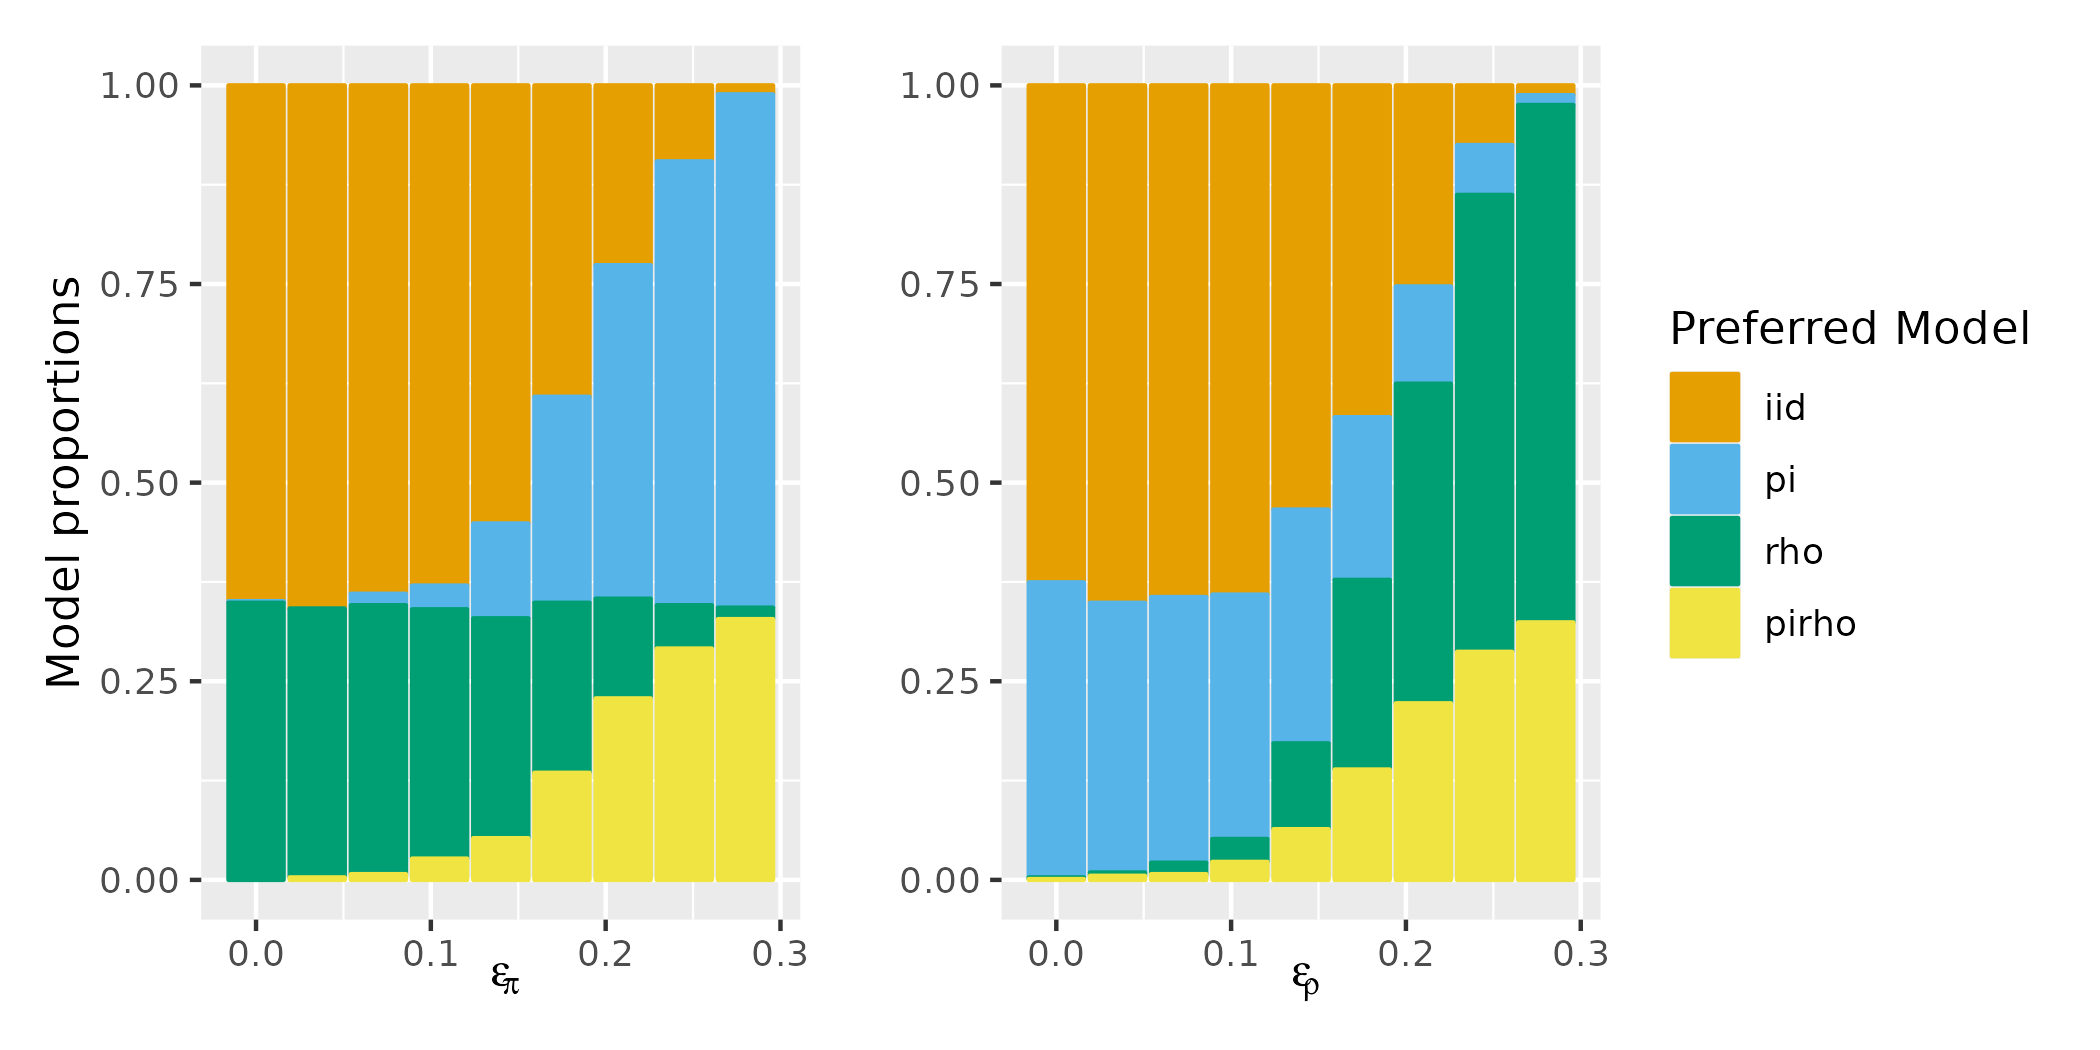
\includegraphics{./Rcodes/simulation/img/plot_model_function_eps.png}
\caption{Plot of preferred model in function of $\eps[\pi]$ and $\eps[\rho]$}
\label{fig:pref_model_func_eps}
\end{figure}

On the figure \ref{fig:pref_model_func_eps} and tables
\ref{tab:pi-model-sel} and \ref{tab:rho-model-sel}, one can see that
there is a turning point around \(\eps[\pi] = 0.2\) (resp.
\(\eps[\rho] = 0.2\)), before which \(iid\text{-}colBiSBM\) and
\(\rho\text{-}colBiSBM\) (resp. \(\pi\text{-}colBiSBM\)) are selected
most of the times and after \(0.2\) the \(\pi\text{-}colBiSBM\) (resp.
\(\rho\text{-}colBiSBM\)) and \(\pi\rho\text{-}colBiSBM\) gets more and
more selected, highlighting our capacity to recover the simulated
structure.

Please note that when ``Recovered \(Q_1\)(or \(Q_2\))'' is not an
integer it's because some procedures returned a value other than 3.
